% !TEX root = ./main.tex
\begin{figure}[h]
    \centering
    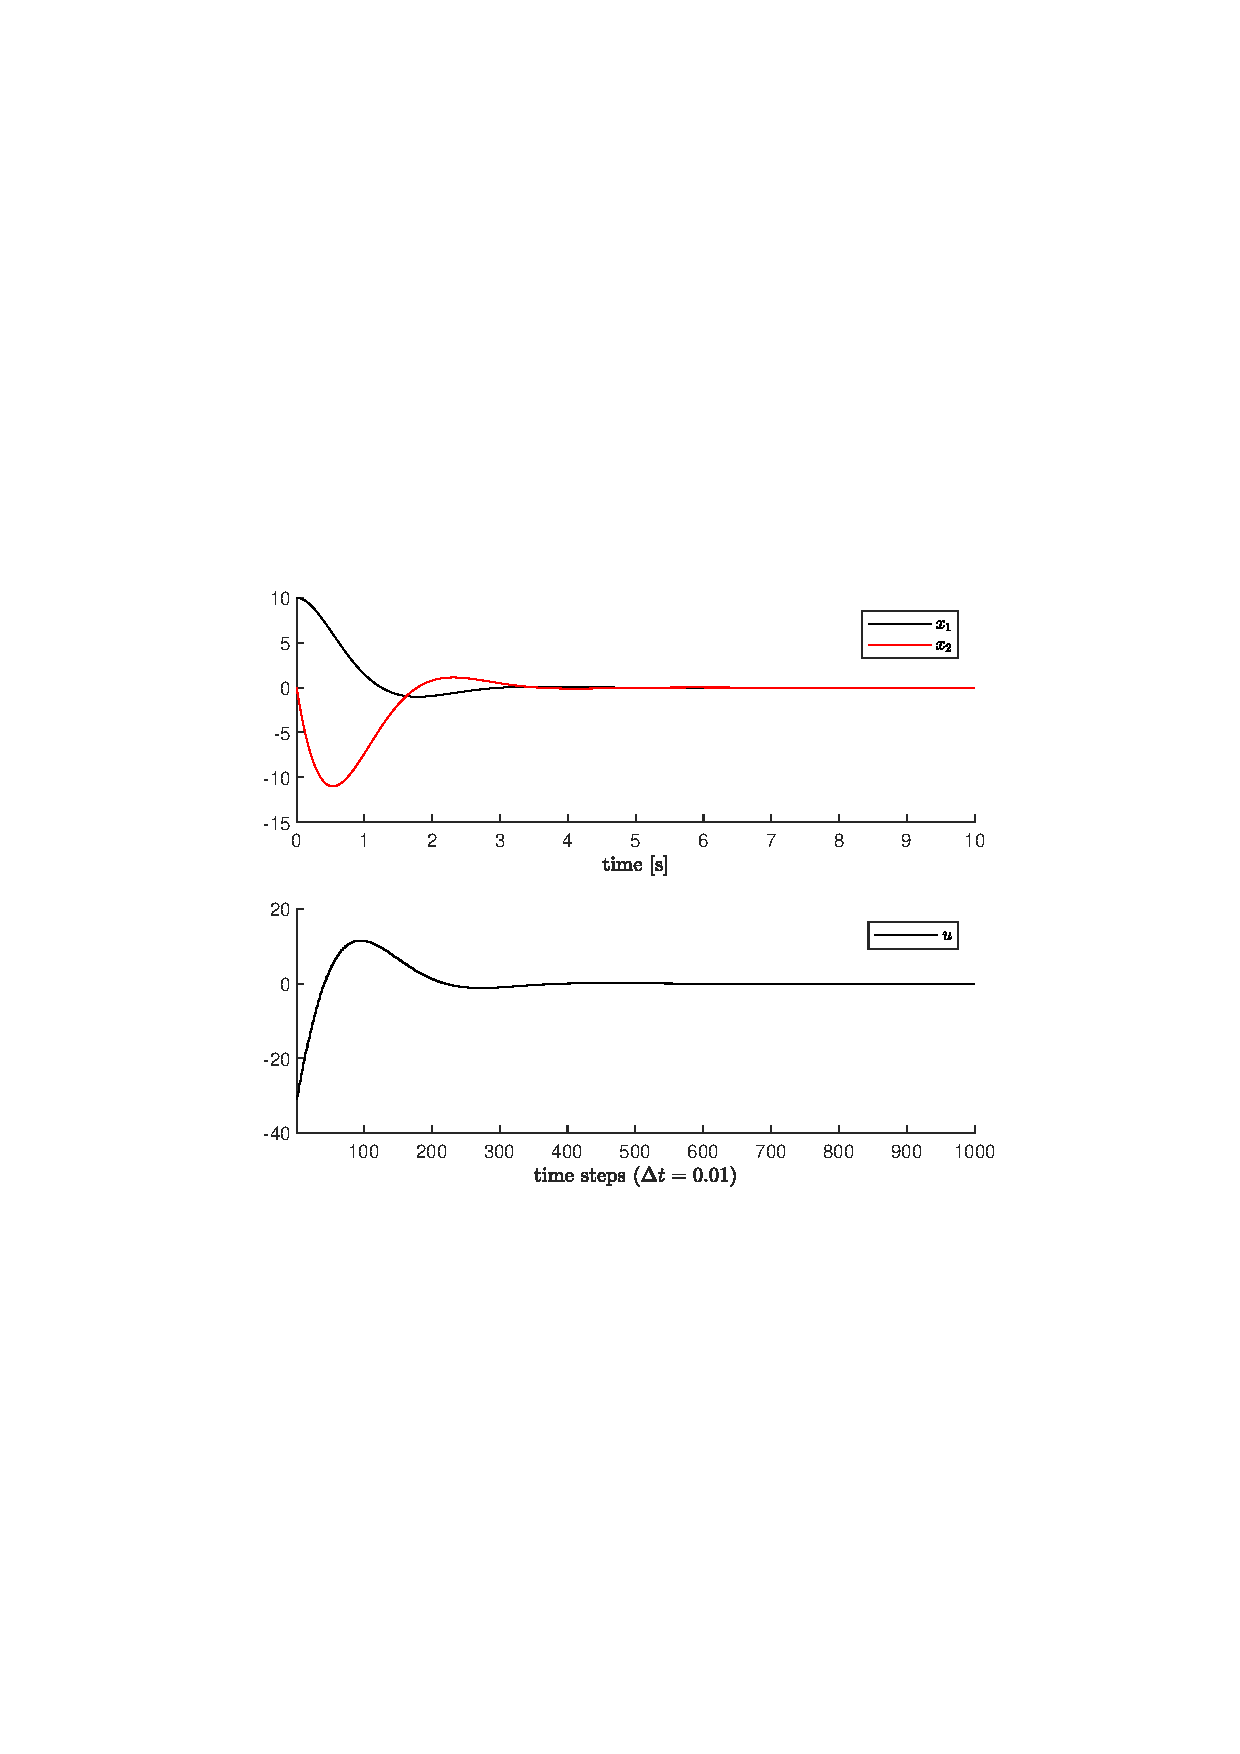
\includegraphics[width=0.8\textwidth]{2_1.pdf}
    \caption{Plots of the resulting $x(t)$ and $u(t)$.}
\end{figure}
\begin{center}
    \begin{tabular}{ |p{1cm}||p{2cm}|p{2cm}|p{2cm}|p{2cm}||p{2cm}|  }
        \hline
        \multicolumn{6}{|c|}{Pertubation $\zeta\left(z(t), v(t)\right)$ and resulting directional derivative $DJ\cdot\zeta$} \\
        \multicolumn{6}{|c|}{$v_i(t)=A_i\cdot\sin(B_i\cdot t+C_i)+D_i$}\\
        \multicolumn{6}{|c|}{$dz/dt(t)=A\cdot z(t)+B\cdot v(t)$}\\

        \hline
        $i$& $A_i$ & $B_i$ &$C_i$ & $D_i$ & $DJ\cdot\zeta_i$\\
        \hline
        1   & 10.00    & 0.1 &  $0$ & 1 & 5.93E-05 \\
        2  & 5.00    & 0.2 &  $2\pi\cdot1/9$ & 2 & 4.50E-05    \\
        3 & $3.3\overline{3}$    & 0.3 &  $2\pi\cdot2/9$ & 3 & 7.93E-07\\
        4  & 2.50    & 0.4 &  $2\pi\cdot3/9$ & 4 & -9.05E-07\\
        5 & 2.00    & 0.5 &  $2\pi\cdot4/9$ & 5 & 4.11E-05\\
        6 & $1.6\overline{6}$    & 0.6 &  $2\pi\cdot5/9$ & 6 &5.86E-05 \\
        7 & 1.43    & 0.7 &  $2\pi\cdot6/9$ & 7 &  3.05E-05 \\
        8 & 1.25    & 0.8 &  $2\pi\cdot7/9$ & 8 & 2.60E-05 \\
        9 & $1.1\overline{1}$    & 0.9 &  $2\pi\cdot8/9$ & 9 & 7.70E-05 \\
        10 & 1.00    & 0.10 &  $2\pi$ & 10 & 1.07E-04 \\
        \hline
       \end{tabular}  
\end{center}